% !TeX spellcheck = de_DE
\documentclass{alex_gp}

\name{Alexander Helbok}
\course{Grundpraktikum}
\hwnumber{Fehlerrechnung}
\spacing{1.8}

\begin{document}
\renewcommand{\labelenumi}{\alph{enumi})}


\begin{mybox}{Richtiges Runden}
	\centering \( x = 1.2736 \unit{m};\qquad \alpha_x = 0.25034 \unit{m} \)
	\tcblower
	\begin{enumerate}
		\item \( \left(1.274 \pm 0.250 \right) \unit{m} \qquad \xmark \)  Nur eine signifikante Stelle im Fehler
	\tcbline*
		\item \( \left(1.3 \pm 0.3 \right) \qquad \xmark \)  Keine Einheiten!
	\tcbline*
		\item \( 1273 \pm 250 \unit{mm} \qquad \xmark \)  Nur eine signifikante Stelle im Fehler
	\tcbline*
		\item \( 1.3(3) \unit{m} \qquad \cmark \)
	\tcbline*
		\item \( 1.3(25) \unit{m} \qquad \xmark \)  Nur eine signifikante Stelle im Fehler
	\tcbline*
		\item \(  (1.3 \pm 0.25034) \unit{m} \qquad \xmark \)  Nur eine signifikante Stelle im Fehler
	\end{enumerate}
\end{mybox}

\begin{mybox}{Fehlerfortpflanzung}
	\centering \( x = (17.4 \pm 0.3) \unit{V};\quad y = (9.3 \pm 0.7) \unit{V} \)
	\tcblower
	\begin{enumerate}
		\item \( z = x - y = 8.1(8) \unit{V} \)
	\tcbline*
		\item \( z = 12x + 3y = 237(4) \unit{V} \)
	\tcbline*
		\item \( z = 5xy = 8.1(6) \cdot 10^{2} \unit{V^2} \)
	\tcbline*
		\item \( z = \tfrac{y^3}{x^2} = 2.7(6) \unit{V} \)
	\tcbline*
		\item \( z = x^2 + 3y^2 = 5.6(4) \cdot 10^{2} \unit{V^2}\)
	\tcbline*
		\item \( z = \arcsin(\tfrac{y}{x}) = 0.56(5) \)
	\tcbline*
		\item \( z = \sqrt{3xy} = 22.0(9) \unit{V} \)
	\tcbline*
		\item \( z = \ln(\tfrac{y}{x}) = -0.63(8) \)
	\tcbline*
		\item \( z = \tfrac{x}{y^2} + \tfrac{y}{x^2} = 0.23(3) \unit{1/V} \)
	\tcbline*
		\item \( z = 2\sqrt{\tfrac{y}{x}} = 1.46(6) \)
	\end{enumerate}
\end{mybox}

\begin{mybox}{Beispiel: Bestimmung der Fallbeschleunigung \( g \)}
	\vspace{-0.75cm}
	\begin{align*}
		&x_1 = 5.000(1) \unit{m};\quad &x_2 &= 17.000(1) \unit{m};\quad &t_x &= 77283.5(1) \unit{\micro\s} &&\\
		&z_1 = 0 \unit{m};\quad &z_2 &= 20.000(1) \unit{m};\quad &t_z &= 129335.3(1) \unit{\micro\s} &&
	\end{align*} 
	\tcblower
	\begin{enumerate}
		\item \( v = \tfrac{x_2 - x_1}{t_x} = 155.27(2) \unit{\v} \)
	\tcbline*
		\item \( x(t) = x_0 + v_0t + \tfrac{1}{2}a_0t^2 \)
		\begin{flalign*}
			x(t_z) - x(0) &= (z_2 - z_1) + vt_z + \tfrac{1}{2}gt_z^2 &&\\[2ex]
			g &= 2\tfrac{(z_2 - z_1) - vt_z}{t_z^2} = -9.8(3) \unit{\a} &&
		\end{flalign*}
	\tcbline*
		\item Das Experiment misst die Erdbeschleunigung \( g \) zwar etwas ungenau, das Ergebnis verträgt sich aber gut mit dem Literaturwert. Um die Unsicherheit in \( g \) zu vermindern, müsste man in genauere Distanzmessungen investieren, da die Unsicherheiten in \( x_1 \) und \( x_2 \) über \( 99 \% \) des Gesamtfehlers in \( v \) und ungefähr \( 85 \% \) in \( g \) ausmachen. Die Zeit hingegen trägt bei beiden Ergebnissen weniger als \( 1 \) Prozent bei und ist daher verhältnismäßig sehr genau.\par
		Indem man das Objekt fallen lässt, kann man den Fehler in \( v \) eliminieren, und so einen genaueren Wert für die Erdbeschleunigung ermitteln.
	\end{enumerate}
\end{mybox}

\begin{mybox}{Plotten von Daten mit linearem Fit}
	\centering \[ \chi^2 = \sum_{i}^{N} \tfrac{\left(y_i - y(x_i)\right)^2}{\sigma_i^2} = \sum_{i}^{N} \tfrac{\left(y_i - ax_i - b \right)^2}{\sigma_i^2} \]
	\tcblower
	\begin{enumerate}
		\item Die Größe \( \chi^2 \) (Quadratsumme der fehlernormierten Abweichungen) kann herangezogen werden, um die Güte einer Anpassung zu quantifizieren, wobei es von den Fitparametern abhängt. Wollen wir dieses Chi-Quadrat minimieren müssen wir das Minimum von \( \chi^2(a,b) \) in der \( a, b \) Ebene finden indem wir die Nullstellen der partiellen Ableitungen ermitteln.
		\begin{equation}
			\pdv{\chi^2(a,b)}{a} = \sum_{i}^{N} x_i \tfrac{y_i - ax_i - b}{\sigma_i^2} = 0;\quad 
			\pdv{\chi^2(a,b)}{b} = \sum_{i}^{N} \tfrac{y_i - ax_i - b}{\sigma_i^2} = 0 
		\end{equation}
	\tcbbreak
		Jetzt haben wir zwei Gleichungen mit zwei Unbekannten und wir können durch Umformen und Einsetzen analytische Lösungen für \( a \) und \( b \) finden.
		\begin{empheq}[box=\fbox]{align}
			\label{eqn:a}
			a = \frac{N\sum_{i}x_iy_i - \sum_{i}x_i \sum_{i}y_i}{N\sum_{i}x_i^2 - \left(\sum_{i}x_i\right)^2};\quad 
			b = \frac{\sum_{i}x_i^2 \sum_{i}y_i - \sum_{i}x_i \sum_{i}x_iy_i}{N\sum_{i}x_i^2 - \left(\sum_{i}x_i\right)^2} &&
		\end{empheq}
	\tcbline*
		\item Setzt man jetzt Zahlen in Gleichungen \ref{eqn:a} ein erhält man die folgenden Werte:
		\begin{flalign*}
			a &\approx 0.034 \unit{V/cm} &&\\
			b &\approx 0.086 \unit{V} &&
		\end{flalign*}
	\tcbline*
		\item Die von SciPy berechnete Fitparameter stimmen den manuell berechneten überein, was andeutet, dass das Fitprogramm die gleiche Formel verwendet.
		\begin{figure}[H]
			\vspace{-1cm}
			\centering
			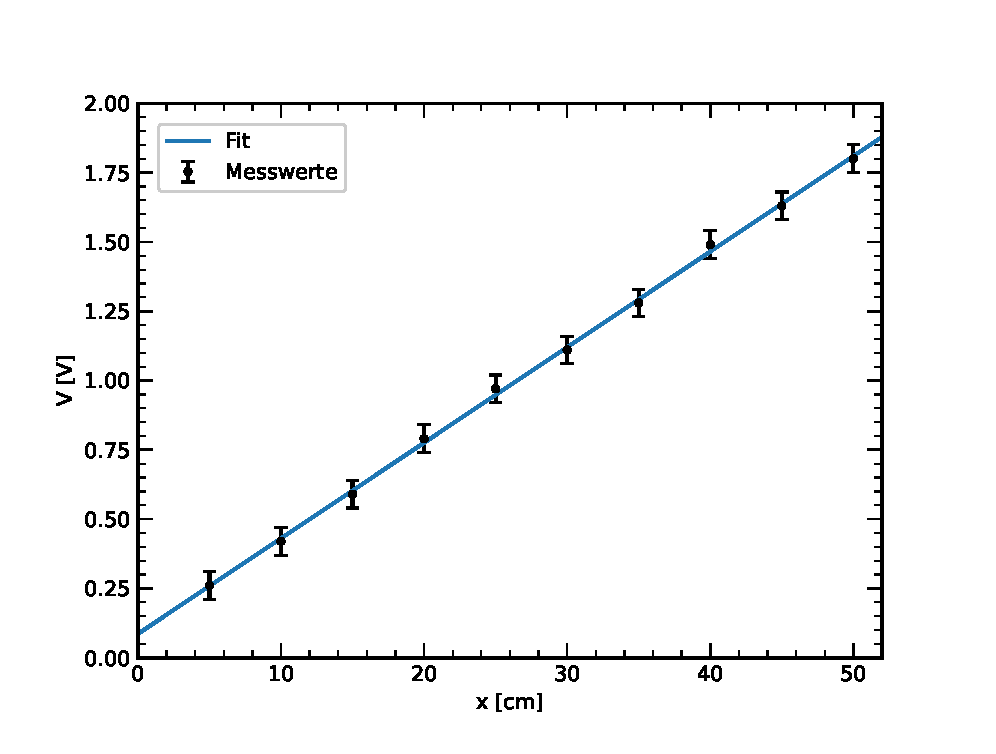
\includegraphics[width=0.75\textwidth]{Fehlerrechnung_1.eps}
			\caption{Die Spannung an verschiedenen Orten gemessen. Die Fehlerbalken stellen einen \( 1 \sigma \) Standardfehler dar. Zudem wurde eine Gerade angepasst.}
		\end{figure}
	\tcbline*
		\item Um die Fehler der beiden Fitparameter zu berechnen wurde das \( \Delta\chi^2 \) als Abweichung vom optimalen Chi-Quadrat gewählt, wenn man \( a \) oder \( b \) variiert. Dabei stellen \( \delta a \) und \( \delta b \) die Differenz zwischen dem Optimalen Fitwert und dem variierten Wert dar.\par
		Trägt man das \( \Delta\chi^2 \) in Abhängigkeit von \( a \) und \( b \) auf erhält man eine Ellipse (Siehe Abbildung \ref{fig:ell}), welche im unkorrelierten Fall (da Korrelation erst im der nächsten Aufgabe eingeführt wird nehme ich unkorrelierte Parameter an) nicht geneigt ist und durch die Gleichung 
		\begin{equation}
			\frac{\delta a^2}{\alpha_a^2} + \frac{\delta b^2}{\alpha_b^2} = r
		\end{equation}
		beschrieben wird.\par
		Unter Annahme einer Gaußverteilung kommt man darauf, dass ein \( \Delta\chi^2 \) von Eins gerade einer Abweichung von \( 1\sigma \) in den Fitparametern entspricht also setzen wir
		\begin{equation}
			\label{eq:delta}
			\Delta\chi^2 = \sum_{i}^{N} \tfrac{\left(y_i - ax_i - b \right)^2}{\sigma_i^2} - \sum_{i}^{N} \tfrac{\left(y_i - \bar{a}x_i - \bar{b} \right)^2}{\sigma_i^2} = \frac{\delta a^2}{\alpha_a^2} + \frac{\delta b^2}{\alpha_b^2} = 1 \\
		\end{equation}
		\( \delta a \) und \( \delta b \) wurden numerisch ermittelt, indem ein Parameter am Optimalwert festgehalten und der Andere so lange erhöht wurde bis \( \Delta\chi^2 = 1 \). So erhält man 
		\begin{equation}
			\delta a \approx 0.00049 \unit{V/cm};\quad \delta b \approx 0.015 \unit{V}
		\end{equation}
			Fixiert man nun \( a, b \) auf \( \bar{a}, \bar{b} \) und setzt das in \ref{eq:delta} ein, fällt ein Bruch weg und man erhält, dass \( \alpha_a = \delta a \) und \( \alpha_b = \delta b \). \par
			Also gilt:
		\begin{flalign*}
			\alpha_a &= \delta a \approx 0.00055 \unit{V/cm} &&\\
			\alpha_b &= \delta b \approx 0.015 \unit{V} &&
		\end{flalign*}
		\begin{figure}[H]
			\vspace{-0.5cm}		
			\centering
			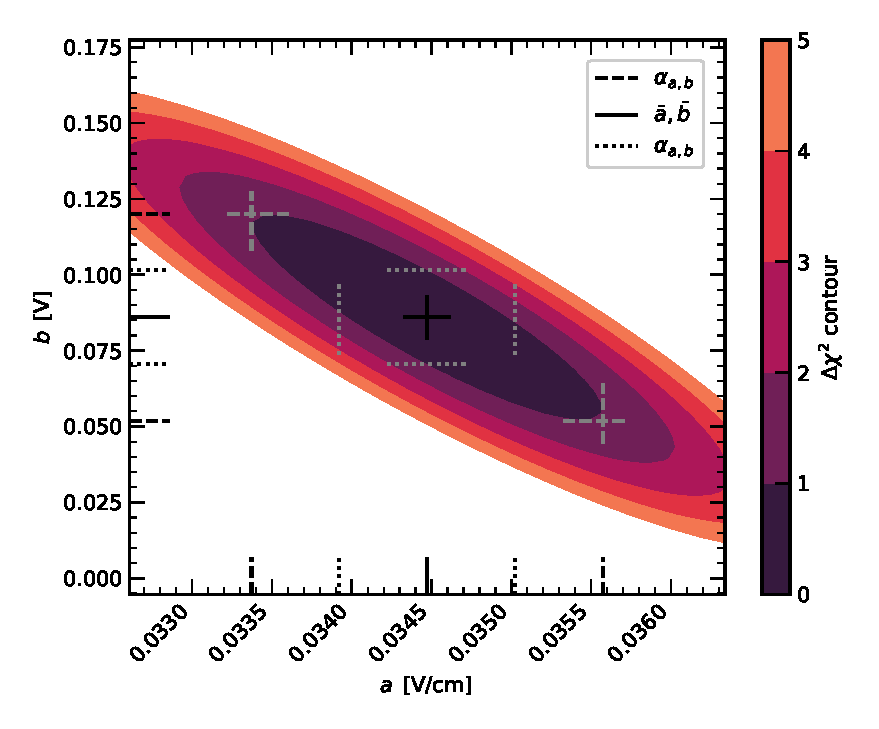
\includegraphics[width=\textwidth]{heat.eps}
			\caption{Fehlerellipse mit farblich hervorgehobenen \( \Delta\chi^2 \) Konturen. Außerdem wurden der optimale Wert für \( a \) und \( b \) (durchgezogen), dessen Fehler (strichliert) und die Fehler ohne Korrelation (gepunktet) eingetragen.}
			\label{fig:ell}
		\end{figure}
	\tcbline*
		\item Das Fitprogramm (SciPy) gibt folgende Fehler für die Parameter aus:
		\begin{flalign*}
			\alpha_a &\approx 0.0011 \unit{V/cm} &&\\
			\alpha_b &\approx 0.034 \unit{V} &&
		\end{flalign*}
		Die Fehler stimmen nicht überein (circa um den Faktor 2 zu klein). Das lässt sich dadurch erklären, dass der Ansatz über das \( \Delta\chi^2 \) und der Fehlerellipse so nur dann gilt, wenn die Parameter unkorreliert sind. Das sind sie aber nicht (\( r \approx -0.89 \)). Das Fitprogramm erkennt die Korrelation und berechnet die Fehler dementsprechend korrekt.
	\tcbline*
		\item Man könnte die Fitparameter \( a, b \) für \( x = \bar{x} - \alpha_x, x = \bar{x} \) und \( x = \bar{x} + \alpha_x \) mit Gleichungen \ref{eqn:a} berechnen und so Werte für \( \bar{a}, \bar{b}, \alpha_a, \alpha_b \) ermitteln. \par
		Alternativ könnte man bootstrapping verwenden, also aus dem Datensatz viele synthetische Datensätze (ohne Fehler) durch „ziehen mit zurücklegen“ generieren (wobei jeder gezogene Wert zufällig im Intervall \( \pm \sigma_x \) und \( \pm \sigma_y \) variiert wird) und auf diese die bekannten Formeln anwenden. Unter Annahme einer Normalverteilung kann man dann Mittelwert und Standardabweichung für die Fitparameter berechnen.
	\end{enumerate}
\end{mybox}

\begin{mybox}{Korrelierte Variablen}
	\centering \( y = ax + b;\quad \bar{a} = 3.77;\quad \bar{b} = 1.58;\quad \sigma = 
	\begin{pmatrix}
		0.033 & 0.019 \\
		0.019 & 0.009
	\end{pmatrix} \)
	\tcblower
	Um den Schnittpunkt mit der x-Achse zu finden muss man die Funktionsgleichung \linebreak \( y = ax + b \) gleich Null setzen und erhält dann als besten Schätzwert
	\begin{equation}
		\label{eqn:x}
		\bar{x} = -\tfrac{\bar{b}}{\bar{a}}
	\end{equation}
	Den Fehler von \( x \) erhält man indem man zur Propagationsformel für unkorrelierte Variablen einen Mischterm dazuaddiert, der beide partiellen Ableitungen und die Kovarianz zwischen \( a \) und \( b \) enthält.
	\begin{equation}
		\label{eqn:sigx}
		\sigma_x = \sqrt{\left( \pdv{x}{b} \right)^2 \sigma_{\text{bb}} + \left( \pdv{x}{a} \right)^2 \sigma_{\text{aa}} + 2\sigma_{\text{ab}}\left( \pdv{x}{a} \right)\left( \pdv{x}{b} \right)} 
	\end{equation}
	Setzt man nun Werte in \ref{eqn:x} und \ref{eqn:sigx} ein erhält man
	\begin{equation}
		x = -0.419(9)
	\end{equation}
\end{mybox}
	  
\end{document}